%%% LaTeX Template originaly created by Karol Kozioł (mail@karol-koziol.net) and modified for ShareLaTeX use

\documentclass[a4paper,11pt]{article}

\usepackage[T1]{fontenc}
\usepackage[utf8]{inputenc}
\usepackage{graphicx}
\usepackage{xcolor}
\usepackage[british]{babel}
\usepackage[german=quotes]{csquotes}

%\renewcommand\familydefault{\sfdefault}
%\usepackage{tgheros}
%\usepackage[defaultmono]{droidmono}

\usepackage{amsmath,amssymb,amsthm,textcomp}
\usepackage{enumerate}
\usepackage{multicol}
\usepackage{tikz}

\usepackage{xcolor}

\usepackage{geometry}
\geometry{left=25mm,right=25mm,%
bindingoffset=0mm, top=20mm,bottom=20mm}
\usepackage{graphicx}
\usepackage{subcaption}
\usepackage{mwe}


\linespread{1.3}

\newcommand{\linia}{\rule{\linewidth}{0.5pt}}

% custom theorems if needed
\newtheoremstyle{mytheor}
    {1ex}{1ex}{\normalfont}{0pt}{\scshape}{.}{1ex}
    {{\thmname{#1 }}{\thmnumber{#2}}{\thmnote{ (#3)}}}

\theoremstyle{mytheor}
\newtheorem{defi}{Definition}

% my own titles
\makeatletter
\renewcommand{\maketitle}{
\begin{center}
\vspace{2ex}
{\huge \textsc{\@title}}
\vspace{1ex}
\\
\linia\\
\@author \hfill \@date
\vspace{4ex}
\end{center}
}
\makeatother
%%%

% custom footers and headers
\usepackage{fancyhdr}
\pagestyle{fancy}
\lhead{}
\chead{}
\rhead{}
%\lfoot{Assignment \textnumero{} 5}
\cfoot{}
\rfoot{Page \thepage}
\renewcommand{\headrulewidth}{0pt}
\renewcommand{\footrulewidth}{0pt}
%

% code listing settings
\usepackage{listings}
\lstset{
    language=Python,
    basicstyle=\ttfamily\small,
    aboveskip={1.0\baselineskip},
    belowskip={1.0\baselineskip},
    columns=fixed,
    extendedchars=true,
    breaklines=true,
    tabsize=4,
    prebreak=\raisebox{0ex}[0ex][0ex]{\ensuremath{\hookleftarrow}},
    frame=lines,
    showtabs=false,
    showspaces=false,
    showstringspaces=false,
    keywordstyle=\color[rgb]{0.627,0.126,0.941},
    commentstyle=\color[rgb]{0.133,0.545,0.133},
    stringstyle=\color[rgb]{01,0,0},
    numbers=left,
    numberstyle=\small,
    stepnumber=1,
    numbersep=10pt,
    captionpos=t,
    escapeinside={\%*}{*)}
}

% ref packages
\usepackage{nameref}
% folowing  must be in this order
\usepackage{varioref}
\usepackage{hyperref}
\usepackage{cleveref}

\setlength\parindent{0pt}

%%%----------%%%----------%%%----------%%%----------%%%

\begin{document}

\title{INF273 – Assignment 1}

\author{Lukas Schramm}

\date{\today}

\maketitle

\section*{Task 1a}
The task is to find a good representation of a solution of the \enquote{Liner shipping problem} as seen in figure \ref{fig:task1a}. There is a port in central Europe from which one ship will start to visit a couple of numbered Norwegian ports. There is the possibility to using small vessels which branch away from the main ship at one harbour, delivering goods to some harbours around the region until they get back into the harbour where they came from. The number of small vessels is not upperbounded.\footnote{It is of course formally upperbounded in the way that every vessel should serve at least one port, so there cannot exist more small vessels than ports to visit.}\medskip

My idea

\begin{figure}[h]
\centering
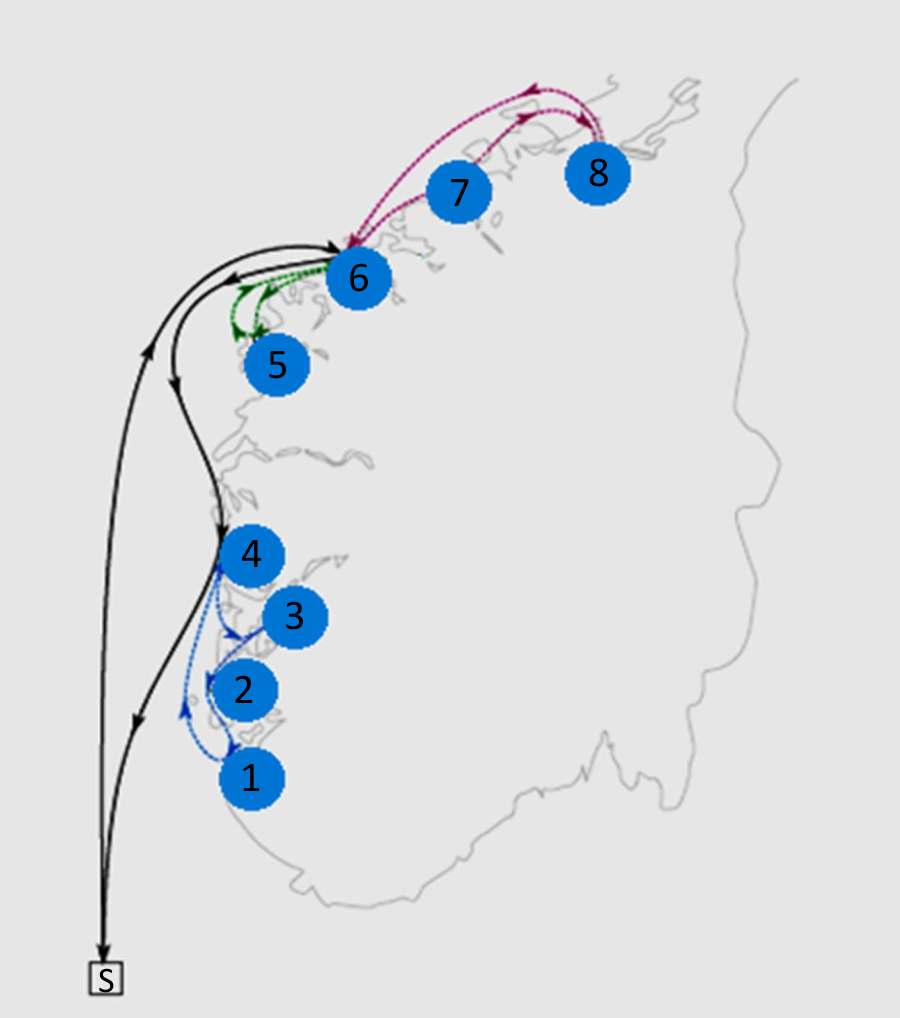
\includegraphics[width=0.5\textwidth]{task1a}
\caption{Illustration of task 1a \enquote{Liner shipping}}
\label{fig:task1a}
\end{figure}

\clearpage


\section*{Task 1b}
The task is to find a good representation of a solution of the \enquote{Truck and drones problem} as seen in figure \ref{fig:task1b}. The task is an extension of the traveling salesperson problem (TSP). Like in TSP, there is a heap of customers to deliver goods to which needs a routing plan from a start point via all the other points back to the origin. The difference for that problem is that there are up to $n$ drones\footnote{$n=2$ in the INF273 course} sitting on the roof of the truck which can deliver one customers each while the truck continues to a different customer. Every drone which visits a customer starts to branch away at a certain point, while they merge again with the truck at the customer afterwards. They cannot return to the original branching point since the track already left that one to visit its next customer. It is not possible to have more than $n$ drones in use at the same time.\medskip

My idea

\begin{figure}[h]
\centering
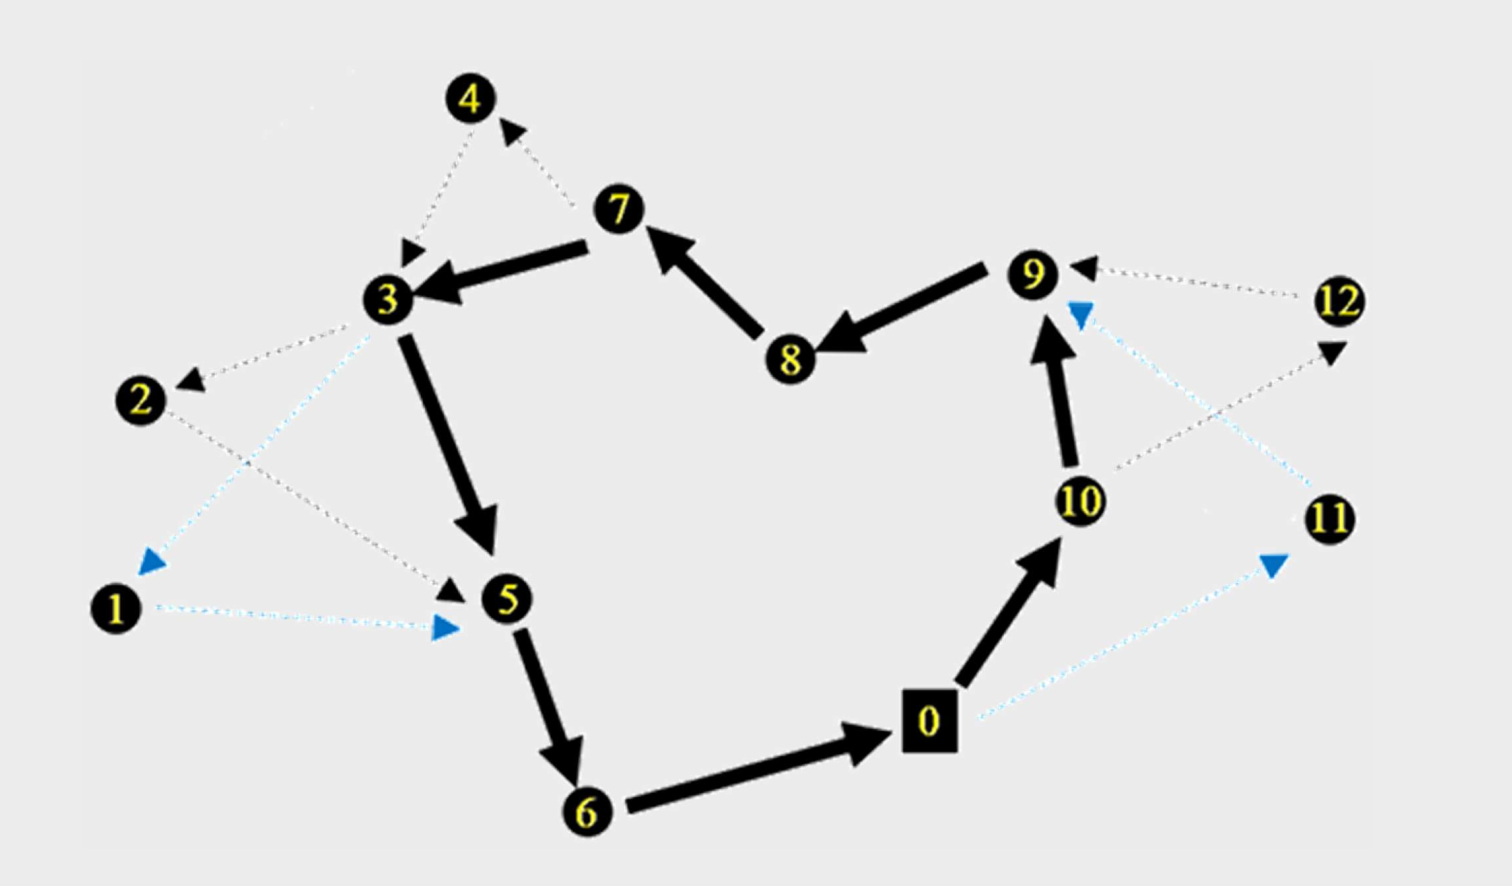
\includegraphics[width=0.5\textwidth]{task1b}
\caption{Illustration of task 1b \enquote{Truck and drones}}
\label{fig:task1b}
\end{figure}


\end{document}